\documentclass{ieeeaccess}
\usepackage{cite}
\usepackage{amsmath,amssymb,amsfonts}
\usepackage{graphicx}
\usepackage{textcomp}
\usepackage{booktabs}
\usepackage{multirow}
\usepackage{xspace}
\usepackage{siunitx}
\sisetup{group-separator={,},group-minimum-digits=4}
\newcommand{\skysim}{SkySim\xspace}
\graphicspath{{../figs/}{./}}
\makeatletter\@ifundefined{xfigwd}{\newdimen\xfigwd\xfigwd=0pt}{}\makeatother

\begin{document}
\history{Date of publication xxxx 00, 0000, date of current version xxxx 00, 0000.}
\doi{10.1109/ACCESS.2026.DOI}

\title{SkySim: A Browser-Native, CPU-Only Multirotor Simulator with Blade-Element Aerodynamics and Lockstep Firmware-in-the-Loop}

\author{\uppercase{Vishwa [Surname]}\authorrefmark{1}}
\address[1]{Independent Researcher, Negombo, Sri Lanka (e-mail: [email])}

\markboth
{[Surname] \headeretal: SkySim: A Browser-Native, CPU-Only Multirotor Simulator}
{[Surname] \headeretal: SkySim: A Browser-Native, CPU-Only Multirotor Simulator}

\corresp{Corresponding author: Vishwa [Surname] (e-mail: [email]).}

\begin{abstract}
Testing autonomy algorithms for multirotor drones usually means installing a
Linux-centric simulation stack, a game engine, or a GPU-bound parallel
simulator. Each of these is a barrier for students, independent researchers,
and teams that only have ordinary laptops. We present \skysim, an open-source
multirotor simulator built around a single dependency-free C++20 physics core.
The same source compiles to a native Godot~4 extension for desktop use, to a
shared library for in-process Python training, and to WebAssembly for
zero-install use in a web browser. The core combines blade-element rotor
aerodynamics with momentum inflow, a first-order motor model, ground effect,
an envelope-based vortex-ring-state model, the ISA atmosphere, Dryden
turbulence, and a LiPo pack model whose sagging voltage limits motor thrust.
Stock ArduPilot and PX4 firmware fly the simulated vehicle through lockstep
JSON and MAVLink bridges. We evaluate the core against UIUC wind-tunnel data for
an APC~10$\times$4.7 propeller. With the propeller's chord and twist mapped onto
\skysim's parameters, the uncalibrated model underpredicts the thrust
coefficient by 34\%. A single collective-pitch offset of $3.75^\circ$, fitted on
thrust alone, brings the mean thrust error to $-0.5$\% and predicts the power
coefficient within $+11$\% on average. We also report a sign error in the axial
inflow term that turned heave damping into anti-damping. It was found through
closed-loop firmware testing and is corrected here. On one 2.1\,GHz server vCPU
the core runs at about 550$\times$ real time natively and 670$\times$ under a
JavaScript engine's WebAssembly runtime. Trajectories agree to within
$1.2\times10^{-14}$\,m across native and WebAssembly builds over 60\,s of
turbulent flight. Small neural policies trained from scratch in 18\,min on two
vCPUs, with no GPU, by both evolution strategies and PPO, hold position more
tightly than a hand-tuned cascaded PID controller (median final error
0.024\,m against 0.133\,m). We state the main limitation plainly: no sim-to-real transfer
result exists yet.
\end{abstract}

\begin{keywords}
Aerial robotics, blade element theory, drone simulation, firmware-in-the-loop,
multirotor, open-source software, reinforcement learning, software-in-the-loop,
unmanned aerial vehicles, WebAssembly.
\end{keywords}

\titlepgskip=-21pt

\maketitle

%===========================================================================
\section{Introduction}
\label{sec:introduction}
\PARstart{S}{imulation} is where most autonomy algorithms for multirotor drones
are first written, tuned, and broken. The tools commonly used for this work are
powerful but heavy. Gazebo-based stacks~\cite{koenig2004gazebo,furrer2016rotors}
are built around Linux and ROS. Photorealistic simulators such as
AirSim~\cite{shah2018airsim} and Flightmare~\cite{song2020flightmare} depend on
the Unreal or Unity game engines. The recent generation of massively parallel
learning environments, such as Aerial~Gym~\cite{kulkarni2025aerialgym} and
OmniDrones~\cite{xu2024omnidrones}, achieves very high throughput by running on
NVIDIA GPUs through Isaac~Gym or Isaac~Sim. Each choice is reasonable for its
target user. Together they leave a gap: there is no simulator that a student
can open by visiting a URL, that runs on the CPU of an ordinary laptop, that
models the rotor aerodynamics behind hover, climb, descent and ground effect,
and that still connects to the production autopilots, PX4~\cite{meier2015px4}
and ArduPilot~\cite{ardupilot}, that the same student will later fly.

\skysim is an attempt to fill that gap. Its central design decision is a
\emph{single physics core}: a set of header-only C++20 subsystems with no engine
dependencies. It is compiled unchanged into three deployment targets: a
Godot~4~\cite{godot} GDExtension (rendering, sensors, scenes), a native shared
library (headless and in-process Python use), and a WebAssembly
module~\cite{haas2017wasm} (browser use). Because all three evaluate the same
rotor, atmosphere, battery and controller code, a policy or controller tested
in the browser sees the same force models as one trained headless or flown by
firmware on the desktop. The headless library and the browser build also share
the rigid-body integrator, so their trajectories match to round-off; the Godot
host integrates the same forces with the engine's own solver.

This paper makes the following contributions:
\begin{enumerate}
\item An architecture that shares one dependency-free physics core across a game
engine, a native library and the browser, with the measured consequence that
native and WebAssembly trajectories agree to within $10^{-14}$\,m
(Section~\ref{sec:arch}, \ref{sec:det}).
\item A real-time rotor model combining blade-element theory with momentum
inflow, ground effect, vortex ring state, ISA atmosphere, Dryden turbulence and a
voltage-coupled battery. Its simplifications are stated explicitly
(Section~\ref{sec:physics}).
\item An external validation of the rotor model against UIUC wind-tunnel data,
including an independent reference BEMT that separates parametrisation error
from aerofoil-model error (Section~\ref{sec:val-static}).
\item A case study showing that closed-loop firmware-in-the-loop testing exposed
a sign error in the axial inflow that reversed heave damping. Unit tests had not
caught it (Section~\ref{sec:val-axial}).
\item Lockstep bridges through which unmodified ArduPilot and PX4 fly the
simulated vehicle (Section~\ref{sec:sitl}), and a CPU-only learning experiment
(Section~\ref{sec:rl}).
\end{enumerate}

All code, data and figure scripts are released under the MIT
licence~\cite{skysimrepo}. We have tried to be careful about what the evidence
supports. \skysim has \emph{not} yet been shown to transfer a policy to a
physical vehicle, and Section~\ref{sec:limits} lists the modelling shortcuts a
user should know about.

%===========================================================================
\section{Related Work}
\label{sec:related}

\textbf{Engine-based simulators.} Gazebo~\cite{koenig2004gazebo} with the
RotorS~\cite{furrer2016rotors} MAV models is the reference environment for
PX4 and ArduPilot software-in-the-loop (SITL) testing. RotorS models each rotor
with a thrust and drag torque proportional to the square of rotor speed, plus
first-order motor dynamics. AirSim~\cite{shah2018airsim} and
Flightmare~\cite{song2020flightmare} pair a fast dynamics model with a game
engine renderer for photorealistic perception research.

\textbf{Lightweight and learning-oriented simulators.}
gym-pybullet-drones~\cite{panerati2021learning} exposes quadrotor control to
reinforcement learning (RL) through a Gym interface on the PyBullet physics
engine, with optional ground effect, drag and downwash terms. RotorPy~\cite{folk2023rotorpy}
is a pure-Python simulator with lumped-parameter aerodynamic wrenches, aimed at
education and research. It prioritises transparency and ease of installation,
a goal \skysim shares.

\textbf{GPU-parallel simulators.} Aerial~Gym~\cite{kulkarni2025aerialgym}
builds on NVIDIA Isaac~Gym, and OmniDrones~\cite{xu2024omnidrones} on Isaac Sim.
Both parallelise thousands of vehicles on a GPU, giving throughputs well beyond
any CPU simulator, at the cost of requiring compatible NVIDIA hardware.

\textbf{Positioning.} Table~\ref{tab:compare} summarises the comparison.
\skysim is not faster than GPU simulators and does not render
photorealistically. Its contribution is the combination of zero-install
browser execution, CPU-only operation, a blade-element rotor model, and lockstep
firmware bridges, all sharing one physics core.

\begin{table}[t]
\centering
\caption{Comparison with open-source multirotor simulators, based on their
published descriptions. ``$\omega^2$'' denotes a quadratic thrust-coefficient
rotor model.}
\label{tab:compare}
\setlength{\tabcolsep}{3pt}
\footnotesize
\resizebox{\columnwidth}{!}{%
\begin{tabular}{@{}lcccc@{}}
\toprule
Simulator & Rotor model & Browser & GPU needed & PX4/ArduPilot \\
\midrule
Gazebo + RotorS~\cite{furrer2016rotors} & $\omega^2$ & no & no & yes \\
AirSim~\cite{shah2018airsim} & $\omega^2$ & no & for rendering & yes \\
Flightmare~\cite{song2020flightmare} & $\omega^2$ & no & for rendering & no \\
gym-pybullet-drones~\cite{panerati2021learning} & $\omega^2$ + terms & no & no & no$^{a}$ \\
RotorPy~\cite{folk2023rotorpy} & $\omega^2$ + lumped aero & no & no & no \\
Aerial Gym~\cite{kulkarni2025aerialgym} & $\omega^2$ & no & yes & no \\
OmniDrones~\cite{xu2024omnidrones} & $\omega^2$ & no & yes & no \\
\textbf{\skysim} & \textbf{BET + momentum} & \textbf{yes} & \textbf{no} & \textbf{yes} \\
\bottomrule
\end{tabular}}\\[2pt]
\raggedright\scriptsize $^{a}$The current repository also offers Betaflight SITL.
\end{table}

%===========================================================================
\section{Architecture}
\label{sec:arch}

Fig.~\ref{fig:arch} shows the structure. The physics core consists of
header-only subsystems: atmosphere, blade-element rotor, aerodynamic effects,
flight controller and mixer, sensors, and battery. They depend only on the C++
standard library, and every quantity is in SI units. Two hosts integrate the
rigid body. In the desktop build, \texttt{DroneBody} is a Godot~4.3 GDExtension
node that supplies scenes, rendering, ray-cast depth and segmentation, and the
SITL manager. \texttt{DroneCore} is a standalone host that replaces Godot's
rigid-body solver with its own 6-DoF integrator. It is exposed through a flat C
API, which is compiled with Emscripten~\cite{zakai2011emscripten} for the
browser and as a shared library for Python.

\begin{figure}[t]
\centering
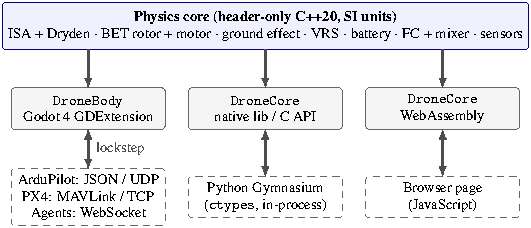
\includegraphics[width=\columnwidth]{fig_arch}
\caption{\skysim architecture. One header-only physics core is compiled into
three hosts. Arrows marked lockstep advance physics by exactly one tick per
exchanged message.}
\label{fig:arch}
\end{figure}

\textbf{Agent protocol.} External algorithms connect to the Godot host over a
WebSocket carrying one JSON object per frame. The protocol is \emph{lockstep}:
the server advances exactly one physics tick (400\,Hz) per action and blocks
until the next action arrives, so a slow algorithm can never fall out of sync
with physics. Observations carry ground-truth state, the full telemetry
dictionary, and optional ray-cast depth and semantic grids. There is a fixed
one-tick actuation latency, as on hardware. WebSocket, rather than raw TCP, was
chosen so that a browser front end can reuse the same protocol.

\textbf{In-process environment.} For CPU-bound training we add a Gymnasium
environment~\cite{towers2024gymnasium} that loads the \texttt{DroneCore} shared
library through \texttt{ctypes} and advances $n$ ticks per call through a
batched entry point (\texttt{skysim\_step\_n}). This removes the per-tick FFI
cost (Section~\ref{sec:perf}).

%===========================================================================
\section{Physics Models}
\label{sec:physics}

We use the Godot convention throughout: world $+Y$ up, body $-Z$ forward. Frames
are converted to NED/FRD at the flight-controller and firmware boundaries.

\subsection{Rigid body}
\texttt{DroneCore} integrates translational dynamics in the world frame and
rotational dynamics in the body frame with semi-implicit Euler at
$\Delta t=2.5$\,ms:
\begin{align}
\dot{\mathbf v} &= \tfrac{1}{m}\big(R(\mathbf q)\,\mathbf F_b + m\mathbf g - (k_1 + k_2\rho\|\mathbf v_r\|)\mathbf v_r\big),\\
\dot{\boldsymbol\omega} &= J^{-1}\big(\boldsymbol\tau_b - \boldsymbol\omega\times J\boldsymbol\omega\big),
\end{align}
where $\mathbf v_r=\mathbf v-\mathbf w$ is airspeed relative to the local wind
$\mathbf w$, $J$ is diagonal, and the attitude quaternion is integrated as
$\dot{\mathbf q}=\tfrac12\mathbf q\otimes(0,\boldsymbol\omega)$ and then
renormalised. The default vehicle is a 1.5\,kg quad-X with 0.127\,m rotors.

\subsection{Rotor aerodynamics}
Each rotor is resolved by blade-element theory over $N=24$ annuli between the
hub cut-out $r_0$ and tip radius $R$. Blade pitch varies linearly,
$\theta(r)=\theta_0+(\theta_t-\theta_0)\frac{r-r_0}{R-r_0}$. With rotor speed
$\Omega$, axial velocity of the hub relative to the air along the thrust axis
$V_c$ (positive in climb), and uniform induced velocity $v_i$, the inflow angle
is $\phi=\operatorname{atan2}(V_c+v_i,\,\Omega r)$. The section forces are
\begin{align}
\alpha &= \theta(r)-\phi,\quad C_l = a\,\alpha,\quad C_d=C_{d0}+C_{d2}C_l^2,\\
dT &= N_b\, \tfrac12\rho V^2 c\,(C_l\cos\phi - C_d\sin\phi)\,dr,\\
dQ &= N_b\, \tfrac12\rho V^2 c\,(C_l\sin\phi + C_d\cos\phi)\,r\,dr,
\end{align}
with $V^2=(\Omega r)^2+(V_c+v_i)^2$ and defaults $a=5.73$\,rad$^{-1}$,
$C_{d0}=0.012$, $C_{d2}=0.08$. The induced velocity satisfies momentum theory,
$T=2\rho A\,|V_c+v_i|\,v_i$. It is solved by three damped fixed-point
iterations per tick using the previous tick's thrust, so across ticks the
inflow relaxes to the coupled BET--momentum solution. Shaft power is
$P=Q\Omega$. Rotor speed follows a first-order ESC lag
($\tau=15$\,ms) toward $\Omega_\text{cmd}=\Omega_\text{max}\sqrt{u}$ for throttle
$u$, with $\Omega_\text{max}=K_V V_\text{supply}$. A gyroscopic term
$I_r\Omega\,\boldsymbol\omega\times\hat{\mathbf z}$ and the reaction torque
complete the wrench.

At hover the default rotor turns at 8000\,RPM, produces 3.68\,N, absorbs
38.6\,W, and has an induced velocity of $v_h=5.44$\,m/s, which equals the
momentum value $\sqrt{T/2\rho A}$. Its figure of merit is 0.52.

\subsection{Ground effect}
Thrust is multiplied by the Cheeseman--Bennett image-source
result~\cite{cheeseman1955ground},
$T_\text{IGE}/T_\text{OGE}=[1-(R/4z)^2]^{-1}$, clamped at $z\ge R/4$. To avoid a
discontinuity, the excess is blended linearly to zero between $z/R=0.25$ and
$z/R=3$ (Fig.~\ref{fig:ground}).

\subsection{Vortex ring state}
\skysim uses an envelope model rather than a modified-inflow
model~\cite{johnson2005vrs}. With $\mu_d=V_d/v_h$ and $\mu_l=V_\text{lat}/v_h$,
onset severity is
$s^\ast=\big(1-\frac{|\mu_d-0.9|}{0.6}\big)\big(1-\frac{\mu_l}{0.5}\big)$ inside
$0.3<\mu_d<1.5,\ \mu_l<0.5$, and zero elsewhere. The applied severity $s$
follows $s^\ast$ through first-order filters with $\tau=0.5$\,s on entry and
$1.2$\,s on recovery. Thrust is scaled by $1-s(0.25+0.05\,n(t))$, where $n(t)$
is a deterministic two-tone buffeting signal near 2.3\,Hz. The steady
thrust-loss map is shown in Fig.~\ref{fig:vrs}. This is an engineering model of
the \emph{effect} of VRS, not of its inflow physics.

\subsection{Atmosphere and turbulence}
Density, pressure, temperature and viscosity follow the ISA
troposphere~\cite{isa1975} with Sutherland's law. Turbulence is a first-order
Gauss--Markov (Dryden-type~\cite{milhdbk1797}) process per axis,
$x_{k+1}=e^{-\Delta t/\tau}x_k+\sigma\sqrt{2\Delta t/\tau}\,\eta_k$, with
$\tau=L/V_\text{ref}$ and a seeded, deterministic, unit-variance generator. The
default is $\sigma=0.1$\,m/s, $L=200$\,m.

\subsection{Battery and voltage--thrust coupling}
The pack (default 4S, 4000\,mAh, 30\,m$\Omega$) integrates charge from the
current actually drawn by the rotors. For electrical power $P$, open-circuit
voltage $V_\text{oc}(\mathrm{SoC})$ (a monotone LiPo-shaped curve) and internal
resistance $R_\text{int}$, the current is the physical root of
$R_\text{int}I^2 - V_\text{oc}I + P = 0$, and the terminal voltage is
$V=V_\text{oc}-IR_\text{int}$. Peukert derating~\cite{peukert1897} removes charge
faster at high C-rates, and a lumped thermal state models $I^2R$ heating. The
terminal voltage from the previous tick sets each motor's speed ceiling,
$\Omega_\text{max}=K_V V$, which breaks the algebraic loop. Coupling only
\emph{reduces} authority below nominal voltage (14.8\,V), so flights on a
healthy pack are unchanged. Because $T\propto\Omega^2$, a pack at 70\% of
nominal delivers $0.490\times$ full-throttle thrust in our unit test, matching
$0.7^2$.

%===========================================================================
\section{Firmware-in-the-Loop}
\label{sec:sitl}

\textbf{ArduPilot.} \skysim implements ArduPilot's documented JSON physics
backend. SITL sends binary servo frames over UDP, and \skysim (bound to port
9002) replies to the sender with a JSON state message containing IMU,
attitude, position and velocity.

\textbf{PX4.} \skysim implements PX4's Simulator MAVLink
API~\cite{mavlink}. The simulator is the TCP server on port 4560. It streams
\texttt{HIL\_SENSOR} and \texttt{HIL\_GPS} and receives
\texttt{HIL\_ACTUATOR\_CONTROLS}, in lockstep: PX4 advances its clock from the
simulator's timestamps, and the simulator waits for the actuator reply before
stepping physics.

Two practical findings are worth reporting for anyone writing a similar
bridge. First, PX4 marks perfectly noise-free magnetometer and barometer
streams as stale and refuses to arm, so \skysim adds seeded noise. Second, the
magnetic field must match the simulated origin. \skysim takes it from the World
Magnetic Model~\cite{wmm2025}: $(23.0, 5.1, -52.6)\,\mu$T NED for the default
Canberra origin.

\begin{table}[t]
\centering
\caption{Stock-parameter autopilots flying \skysim physics (takeoff to 10\,m,
15\,s hold, land, auto-disarm). Run on 15~Oct.~2026 with the corrected rotor
model.}
\label{tab:sitl}
\footnotesize
\begin{tabular}{@{}lccc@{}}
\toprule
Firmware (configuration) & Hold mean & Peak & Landed \\
\midrule
ArduCopter 4.6.3 (\texttt{copter.parm}) & 9.96\,m & 10.03\,m & yes \\
PX4 v1.15.4 (\texttt{none\_iris}) & 9.99\,m & 10.01\,m & yes \\
PX4 main, v1.17.0-dev (\texttt{none\_iris}) & 9.99\,m & 10.02\,m & yes \\
\bottomrule
\end{tabular}
\end{table}

Table~\ref{tab:sitl} reports headless runs in which each autopilot flew a
scripted mission on its stock parameters. All three held altitude within
0.04\,m of the 10\,m target and landed. The protocol layers are covered by 20
offline unit tests, including a UDP loopback test for the JSON backend.

%===========================================================================
\section{Evaluation}
\label{sec:eval}

All experiments use the corrected core and the harness in
\texttt{paper/eval/}. They ran on a cloud VM with two vCPUs of an Intel Xeon
at 2.1\,GHz, using GCC~13.3, Clang~18.1 and Node.js~22 (V8~12.4). No GPU was
used.

\subsection{Static rotor performance against wind-tunnel data}
\label{sec:val-static}

We compare against the UIUC Propeller Data Site~\cite{uiucpropdb,brandt2011propeller}
static measurements for the APC Slow Flyer 10$\times$4.7. Its diameter, 0.254\,m,
matches \skysim's default rotor. Coefficients follow the UIUC convention,
$C_T=T/(\rho n^2D^4)$ and $C_P=P/(\rho n^3D^5)$, with $n$ in rev/s. \skysim's
parametrisation allows only a constant chord and linear twist, so we set
$c=c(0.75R)=25.0$\,mm, $r_0=0.15R$, and a linear twist fitted to the measured
pitch distribution over $r/R\ge0.3$ (least squares, $27.1^\circ$ at the cut-out
to $4.05^\circ$ at the tip). To separate
parametrisation error from aerofoil-model error, we also implemented an
independent reference BEMT. It solves the annulus-wise inflow with Prandtl tip
loss~\cite{leishman2006principles} on the \emph{full} measured chord and twist,
using the same section coefficients.

Fig.~\ref{fig:static} shows the result. Uncalibrated, \skysim underpredicts
$C_T$ by 33.8\% and $C_P$ by 37.2\% on average. The reference BEMT is lower
still ($C_T=0.072$). This rules out the simplified inflow and parametrisation as
the cause: the deficit comes from the symmetric thin-aerofoil lift law, which
has no zero-lift angle and so ignores the camber of real propeller sections.
For a linear lift curve, a zero-lift angle $\alpha_0$ is exactly equivalent to
adding $-\alpha_0$ to the blade pitch. We therefore fitted a single
collective-pitch offset to the measured $C_T$, giving $+3.75^\circ$. After
calibration, the mean $C_T$ error is $-0.5$\% (maximum 10.8\%). The power
coefficient, which was not fitted, is overpredicted by 10.7\% on average
(maximum 22.6\%, at the lowest RPM). The measured coefficients rise with RPM by
about 23\% over the range, a Reynolds-number effect that a constant-coefficient
section model cannot capture.

\begin{figure}[t]
\centering
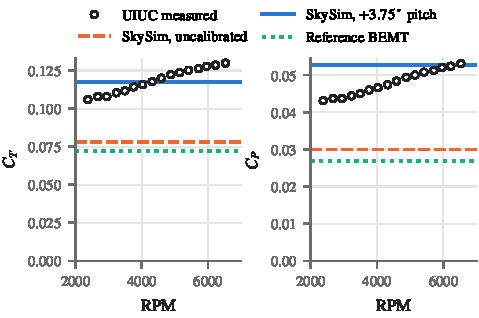
\includegraphics[width=\columnwidth]{fig_static}
\caption{Static thrust and power coefficients of an APC~10$\times$4.7 propeller:
UIUC measurements~\cite{uiucpropdb} against \skysim, uncalibrated and with a
single collective offset fitted on $C_T$, and an independent reference BEMT
using the full measured geometry and the same aerofoil coefficients.}
\label{fig:static}
\end{figure}

\subsection{Axial inflow and a sign error found in the loop}
\label{sec:val-axial}

The released v3.0 core computed the axial inflow velocity as
$V_c=-(\mathbf v_\text{hub}-\mathbf w)\cdot\hat{\mathbf z}_\text{rotor}$. The
sign is wrong: climbing \emph{reduced} the inflow angle and so \emph{increased}
thrust. Fig.~\ref{fig:axial} shows steady thrust at hover RPM against axial
velocity for both versions. Near hover, the corrected model gives
$\partial T/\partial V_c=-0.239$\,N/(m/s) per rotor, the physically expected
heave damping. The original gives $+0.239$. For the 1.5\,kg vehicle this
reverses the rotor contribution to the heave derivative, from
$Z_w=-0.64$\,s$^{-1}$ to $+0.64$\,s$^{-1}$. Because hub velocity includes $\boldsymbol\omega\times\mathbf r$, the
same error also gives the rotor moving upward during a roll or pitch
\emph{more} thrust, so body rates are anti-damped as well.

The error survived the project's unit tests, which checked qualitative trends
such as monotone throttle response, and \texttt{DroneCore}'s own attitude controller masked it. On a 10\,m
altitude step flown with that controller and a simple PID altitude loop, the only visible symptom is a larger overshoot: 14.0\% with the
error and 8.8\% after correction. It became obvious only when unmodified
ArduPilot flew the vehicle. Under ArduCopter's tuned loops it produced an 8\,Hz
attitude limit cycle and a 35\,m altitude overshoot. We think this is a
useful general lesson: for flight dynamics, closed-loop firmware testing works
as a physics test, because production controllers are tuned to the damping
real vehicles have.

\begin{figure}[t]
\centering
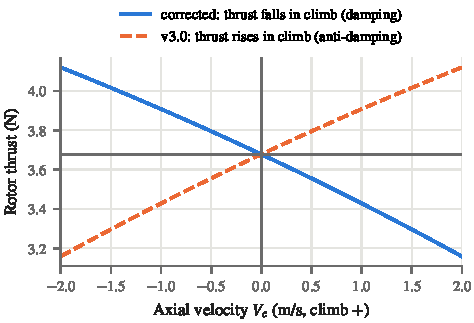
\includegraphics[width=\columnwidth]{fig_axial}
\caption{Steady rotor thrust at hover RPM (8000) against axial velocity, with
the original (v3.0) and corrected inflow sign. The range is limited to
$|V_c|<0.4\,v_h$, where uniform momentum theory is valid.}
\label{fig:axial}
\end{figure}

\subsection{Ground effect and vortex ring state}
Fig.~\ref{fig:ground} compares the applied ground-effect multiplier with
Cheeseman--Bennett. Because of the blend, the model under-applies the classic
result: at $z/R=1$ it adds 4.8\% thrust where Cheeseman--Bennett gives 6.7\%.
In closed-loop hover the required throttle falls from 0.346 out of ground
effect to 0.340 at $z/R=1.42$ ($-1.9$\%), which is consistent with the applied
multiplier. Fig.~\ref{fig:vrs} gives the steady VRS thrust map. The loss peaks
at 25\% at $V_d=0.9\,v_h$ and halves at $\mu_l=0.25$.

\begin{figure}[t]
\centering
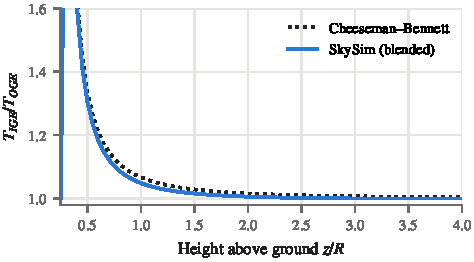
\includegraphics[width=\columnwidth]{fig_ground}
\caption{Ground-effect thrust ratio: Cheeseman--Bennett~\cite{cheeseman1955ground}
against the blended multiplier applied by \skysim.}
\label{fig:ground}
\end{figure}

\begin{figure}[t]
\centering
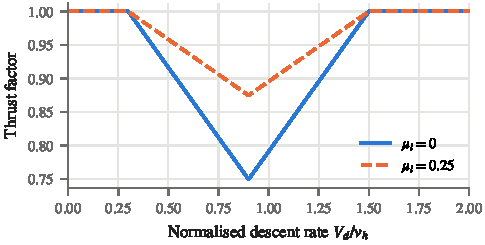
\includegraphics[width=\columnwidth]{fig_vrs}
\caption{Steady thrust factor of the envelope VRS model against normalised
descent rate, for two lateral speed ratios $\mu_l$.}
\label{fig:vrs}
\end{figure}

\subsection{Battery endurance}
A closed-loop 5\,m hover on the default pack (Fig.~\ref{fig:battery}) reaches
the 3.5\,V/cell warning after 18.2\,min and the 3.3\,V/cell cutoff after
21.3\,min. By then it has used 3835\,mAh and 4.1\% state of charge remains. Once
the terminal voltage drops below nominal, at about 12\,min, voltage--thrust
coupling forces the altitude controller to raise hover throttle from 0.345 to
0.439. This is the sluggish end-of-pack behaviour pilots know. The endurance is
the direct consequence of the pack energy (about 59\,Wh) and the model's hover
power (154\,W). Since the model's figure of merit is on the efficient side, it
probably overestimates endurance relative to a real airframe of the same mass.

\begin{figure}[t]
\centering
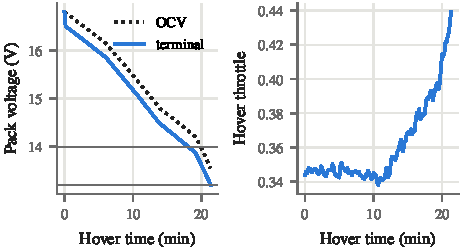
\includegraphics[width=\columnwidth]{fig_battery}
\caption{Hover to cutoff on the default 4S 4000\,mAh pack. Left: open-circuit
and terminal voltage, with warning and cutoff levels. Right: throttle required
to hold altitude as voltage sags.}
\label{fig:battery}
\end{figure}

\subsection{Computational performance}
\label{sec:perf}

Table~\ref{tab:perf} reports the median of three runs of 10 simulated minutes
(240{,}000 ticks) of closed-loop hover with turbulence. The WebAssembly build
was compiled with Clang for \texttt{wasm32-wasi} (via Zig~0.17) and executed by
V8 in Node.js. This is the engine used by Chromium-based browsers, but it is a
proxy, not an in-browser measurement. The WebAssembly build is the fastest
single-thread configuration. We attribute this to differences between the
WASI and glibc implementations of \texttt{exp} and \texttt{sin} rather than to
WebAssembly itself, and have not investigated further. Each instance is
single-threaded, so independent vehicles scale with cores: two instances reach
$1.06\times10^3$ times real time. Through the in-process Gymnasium environment
at a 50\,Hz control rate, Python reaches 20.6k control steps/s, or 165k physics
ticks/s. That is 75\% of raw native throughput, because the batched
\texttt{skysim\_step\_n} call amortises the FFI cost.

\begin{table}[t]
\centering
\caption{Single-vehicle physics throughput on one 2.1\,GHz vCPU (400\,Hz ticks,
closed-loop hover, turbulence on). RTF is the real-time factor.}
\label{tab:perf}
\footnotesize
\begin{tabular}{@{}lrr@{}}
\toprule
Build & ticks/s & RTF \\
\midrule
Native, GCC 13 \texttt{-O3} & \num{218894} & 547 \\
Native, GCC 13 \texttt{-O3 -ffast-math} & \num{233645} & 584 \\
Native, Clang 18 \texttt{-O3} & \num{195180} & 488 \\
WebAssembly (\texttt{wasm32-wasi}, V8 12.4) & \num{266667} & 667 \\
Native GCC, 2 instances on 2 vCPUs & \num{422095} & 1055 \\
Python Gymnasium env via \texttt{ctypes} & \num{165214} & 413 \\
\bottomrule
\end{tabular}
\end{table}

\subsection{Determinism across builds}
\label{sec:det}

Reproducible benchmarks require that a trajectory depends only on its inputs.
We flew a 60\,s scripted manoeuvre (climb, roll and pitch doublets, yaw) with
default turbulence and hashed the full 12-dimensional state at every tick.
GCC \texttt{-O0}, GCC \texttt{-O3} and Clang \texttt{-O3} builds produced
\emph{bit-identical} trajectories, since they share glibc's maths library. The
\texttt{-ffast-math} build and the WebAssembly build differ in the last bits.
Their maximum position deviations from the reference over the whole flight were
$6.0\times10^{-15}$\,m and $1.2\times10^{-14}$\,m, on a trajectory spanning
about 20\,m. All stochastic terms (turbulence, sensor noise, VRS buffeting) are
seeded, so runs are repeatable on any one build. Bit-identical results across
platforms would require a shared maths library.

\subsection{CPU-only policy learning}
\label{sec:rl}

To test the claim that useful learning needs no GPU, we trained a position-hold
policy from scratch with two learners that represent opposite ends of the
design space: OpenAI-style evolution strategies (ES)~\cite{salimans2017es},
implemented in about 150 lines of NumPy with no deep-learning framework, and
proximal policy optimisation (PPO)~\cite{schulman2017ppo} from
Stable-Baselines3~\cite{raffin2021sb3} on PyTorch, forced onto the CPU. The
task starts from a random offset of up to $\pm2$\,m horizontally and $-1.5$ to
$+2$\,m vertically from a 3\,m target, with
random steady wind of up to 2\,m/s per horizontal axis and 0.4\,m/s vertically.
Episodes last 8\,s at 50\,Hz. Both learners use a $12$--$32$--$32$--$4$ tanh
MLP policy (\num{1604} weights) commanding roll, pitch, yaw rate and collective
through \skysim's attitude controller. ES used 24 antithetic pairs, three
episodes per candidate, centred-rank fitness shaping and Adam, with candidates
evaluated in two worker processes. PPO used eight subprocess environments,
observation and reward normalisation, 512-step rollouts per environment, ten
epochs per update with minibatches of 512, a $64$--$64$ value network, an
initial log standard deviation of $-1$ and a learning rate of
$3\times10^{-4}$. These settings were chosen once and not tuned. Each learner received the same budget of
\SI{1100}{s} of wall-clock training time on two vCPUs (PPO excluding the time
spent on validation roll-outs). Both are compared with a hand-tuned cascaded
PID position controller on the same 100 held-out seeds.


Fig.~\ref{fig:es} shows validation return on 20 fixed seeds against training
time. Both learners passed the PID baseline within about two minutes: ES after
70 generations (2.3\,min) and PPO after \num{500000} environment steps
(1.9\,min). Within the 18.3\,min budget, ES completed 500 generations
(\num{72000} episodes, at most 0.23 billion physics ticks), and PPO collected
4.68 million control steps (37.4 million physics ticks). ES thus consumed up
to about six times as much simulated experience as PPO, but needed no
deep-learning framework at all. Table~\ref{tab:es} compares the final policies
with PID on 100 held-out seeds. We count an episode as a success if the
vehicle does not crash and its mean position error over the last 2\,s is
below 0.25\,m.

\begin{table}[t]
\centering
\caption{Position hold on 100 held-out seeds (random start offset and wind),
after 18.3\,min of CPU-only training. Tail error is the mean position error
over the final 2\,s of an episode.}
\label{tab:es}
\footnotesize
\setlength{\tabcolsep}{4pt}
\begin{tabular}{@{}lcccc@{}}
\toprule
Controller & Return & Tail err.\ (median) & Success & Crash \\
\midrule
Cascaded PID & $-0.433$ & 0.133\,m & 98\% & 0\% \\
ES (NumPy MLP) & $-0.245$ & 0.024\,m & 100\% & 0\% \\
PPO (SB3, PyTorch CPU) & $-0.268$ & 0.024\,m & 100\% & 0\% \\
\bottomrule
\end{tabular}
\end{table}

\begin{figure}[t]
\centering
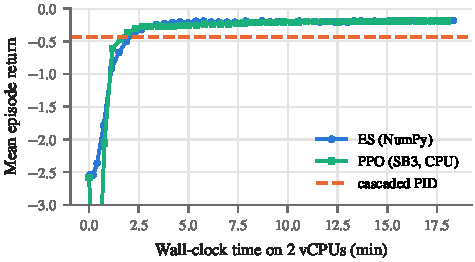
\includegraphics[width=\columnwidth]{fig_es}
\caption{CPU-only training on \skysim: mean validation return on 20 fixed
seeds against wall-clock training time on two vCPUs, for evolution strategies
and PPO, with the cascaded PID baseline for reference. The vertical axis is
clipped at $-3$; PPO's first evaluation after initialisation reached $-5.0$.}
\label{fig:es}
\end{figure}

The two learned policies reach the same median tail error, 0.024\,m, and
neither crashed. The ES policy has the slightly better mean return on the
held-out seeds. The ES and PID results come from one run on the 2.1\,GHz
machine of Section~\ref{sec:eval}; the PPO run was made later on a 2.3\,GHz
vCPU of the same family. Each learner was run with a single seed, so the
comparison between them is indicative only.

This experiment is not a claim that learned policies beat PID control in
general. The PID gains were tuned by hand in a few minutes, and the baseline
has no horizontal integral action, so most of its residual error is the
steady offset caused by wind. A PID controller with wind integrators would
close much of the gap. The claim the experiment supports is narrower: with
either a gradient-free or a standard deep-RL learner, a closed-loop flight
policy can be trained from scratch against \skysim's full rotor model on a
commodity CPU in minutes, without a GPU.


%===========================================================================
\section{Limitations}
\label{sec:limits}

\begin{itemize}
\item \textbf{No sim-to-real result.} No policy or controller developed in
\skysim has yet been shown to transfer to a physical vehicle. The repository
documents a transfer protocol and a results template, but the result itself
remains open.
\item \textbf{Aerofoil model.} Constant, symmetric section coefficients with no
stall or Reynolds dependence. A camber offset recovers static $C_T$, but power
remains about 11\% high, and the RPM trend in Fig.~\ref{fig:static} is not
captured.
\item \textbf{Inflow.} Uniform momentum inflow, with no tip loss, no
non-uniform or dynamic inflow, and no in-plane rotor forces (H-force, blade
flapping) in edgewise flight. Body drag is a lumped linear-plus-quadratic term.
\item \textbf{VRS and ground effect} are effect-level engineering models.
Johnson's modified-inflow model~\cite{johnson2005vrs} and partial ground effect
are natural upgrades.
\item \textbf{Measurement scope.} Browser performance was measured with V8 in
Node.js, not inside browsers. The Godot GDExtension host was not benchmarked
here. The SITL results (Table~\ref{tab:sitl}) come from a separate integration
run, not from this paper's harness.
\item \textbf{Software state.} At the time of writing, the public v3.0 release
still contains the inflow sign error of Section~\ref{sec:val-axial}. The
corrected code and all evaluation scripts are on the \texttt{paper-eval}
branch and should be merged before this work is cited as describing the
release.
\end{itemize}

%===========================================================================
\section{Conclusion}
\skysim shows that one dependency-free physics core can serve a desktop game
engine, headless Python training and a web browser at the same time. The
native and WebAssembly builds agree numerically to $10^{-14}$\,m, and a single
vCPU sustains several hundred times real time. Its blade-element rotor model, calibrated with one
physically motivated parameter, reproduces measured static thrust within about
11\%. Unmodified ArduPilot and PX4 fly the simulated vehicle. The most
instructive result was a failure: a sign error that unit tests missed but that
production firmware exposed within seconds. The next steps are a measured
sim-to-real transfer, a cambered and Reynolds-dependent aerofoil model, and
Johnson-type VRS inflow.

\section*{Data and Code Availability}
Source code, the evaluation harness (\texttt{paper/eval/}), raw CSV data
(\texttt{paper/data/}) and figure scripts are available
at~\cite{skysimrepo} under the MIT licence. The UIUC propeller data are
redistributed with attribution to their source~\cite{uiucpropdb}.

\section*{Acknowledgment}
The author thanks the SkySim contributors and the maintainers of ArduPilot,
PX4 and the UIUC Propeller Data Site. Portions of the software, the evaluation
harness and the text of this article were produced with the assistance of an AI
system (Anthropic Claude). All results were generated by executing the released
code, and the author has reviewed the manuscript and takes responsibility for
its content.

\bibliographystyle{IEEEtran}
\bibliography{refs}

\begin{IEEEbiography}{Vishwa [Surname]}
is the creator and maintainer of SkySim. His work spans AI, computer vision
and autonomy for unmanned aerial vehicles, and he contributes to open-source
robotics projects including gym-pybullet-drones, MAVSDK-Python and AgileRL.
[Complete with education and affiliations.]
\end{IEEEbiography}

\EOD
\end{document}
